%%==================================================
%% chapter01.tex for BIT Master Thesis
%% modified by pinren lu
%% version: 0.1
%% last update: Dec 25th, 2016
%%==================================================
% 第五章 模型改写文本检测系统设计与实现

% 1. 需求分析
% 2. 系统设计
% 3. 系统实现
% 4. 系统展示
% 5. 本章小结

\chapter{模型改写文本检测系统设计与实现}
\label{chap:sys}

本章主要介绍基于模型改写文本检测系统的设计与实现,第三、四章从理论和实验方面验证了本文提出方法的有效性,为了进一步验证方法在实际应用场景中的有效性,本文以提出的模型改写文本检测方法为基础,遵循软件开发过程的基本原则,设计并实现了模型改写文本检测系统,涵盖文本改写和检测模型改写两大文本生成功能。通过该系统,可以进一步提升文本改写的流畅性与多样性、检测模型改写的准确性。本章以需求分析、系统设计、系统实现以及系统功能展示四个部分介绍模型改写文本检测系统。

\section{需求分析}
\label{sec:sys-need}

本文研究的模型改写文本检测系统给自然语言处理领域带来提供了一种新的技术方案,能够有效提升对于学生写作文本是否由 AI 改写的检测能力,本文构建的模型改写文本检测系统旨在给用户提供一个功能完善的、性能优越的模型改写文本检测系统,该系统用户可以为用户提供多样的文本改写服务以及精准的模型文本改写检测服务。接下来将从业务需求和功能需求角度进行详细分析。

\subsection{业务需求分析}
\label{sec:sys-bus-need}

随着人工智能技术的快速发展,文本改写和检测模型改写的需求日益增长。尤其是在教育领域,教师需要对学生的写作进行评估和反馈,而学生也希望能够通过改写工具提升自己的写作能力。因此,本文提出的模型改写文本检测系统应具备以下业务需求:

\begin{itemize}
    \item \textbf{文本改写服务:} 系统应能够提供高质量的文本改写服务,帮助用户提升文本的流畅性和多样性。
    \item \textbf{模型改写检测服务:} 系统应能够准确检测出文本是否经过模型改写,帮助教师评估学生的写作水平。
    \item \textbf{用户友好的界面:} 系统应具备简洁易用的用户界面,方便用户进行操作。
    \item \textbf{高性能和稳定性:} 系统应具备良好的性能和稳定性,能够处理大量的文本数据。
    \item \textbf{安全性和隐私保护:} 系统应确保用户数据的安全性和隐私保护,防止数据泄露。
    \item \textbf{可扩展性:} 系统应具备良好的可扩展性,能够根据需求进行功能扩展和升级。
    \item \textbf{多平台支持:} 系统应能够在不同的平台上运行,包括桌面和移动设备。
    \item \textbf{实时反馈:} 系统应能够提供实时的文本改写和检测反馈,帮助用户及时了解文本的质量和改写效果。
    \item \textbf{用户管理:} 系统应具备用户管理功能,支持用户注册、登录、权限管理等操作。
\end{itemize}

\subsection{功能需求分析}
\label{sec:sys-func-need}

本文从用户和管理员两个角度进行了系统的功能分析,以全面了解系统在不同用户身份下的需求和功能要求。用户功能需求分析从系统提供的服务和功能出发,如用户注册、登录、包括文本改写和检测文本改写功能以及用户历史信息管理等,以确保用户能够顺利地使用系统并获得良好的体验。管理员功能需求分析侧重于系统的管理和维护功能,如用户管理、功能管理、模型管理以及文本改写信息管理等,以确保系统能够高效稳定地运行,并及时处理用户反馈和问题。

\begin{figure*}[htb]
    \centering
    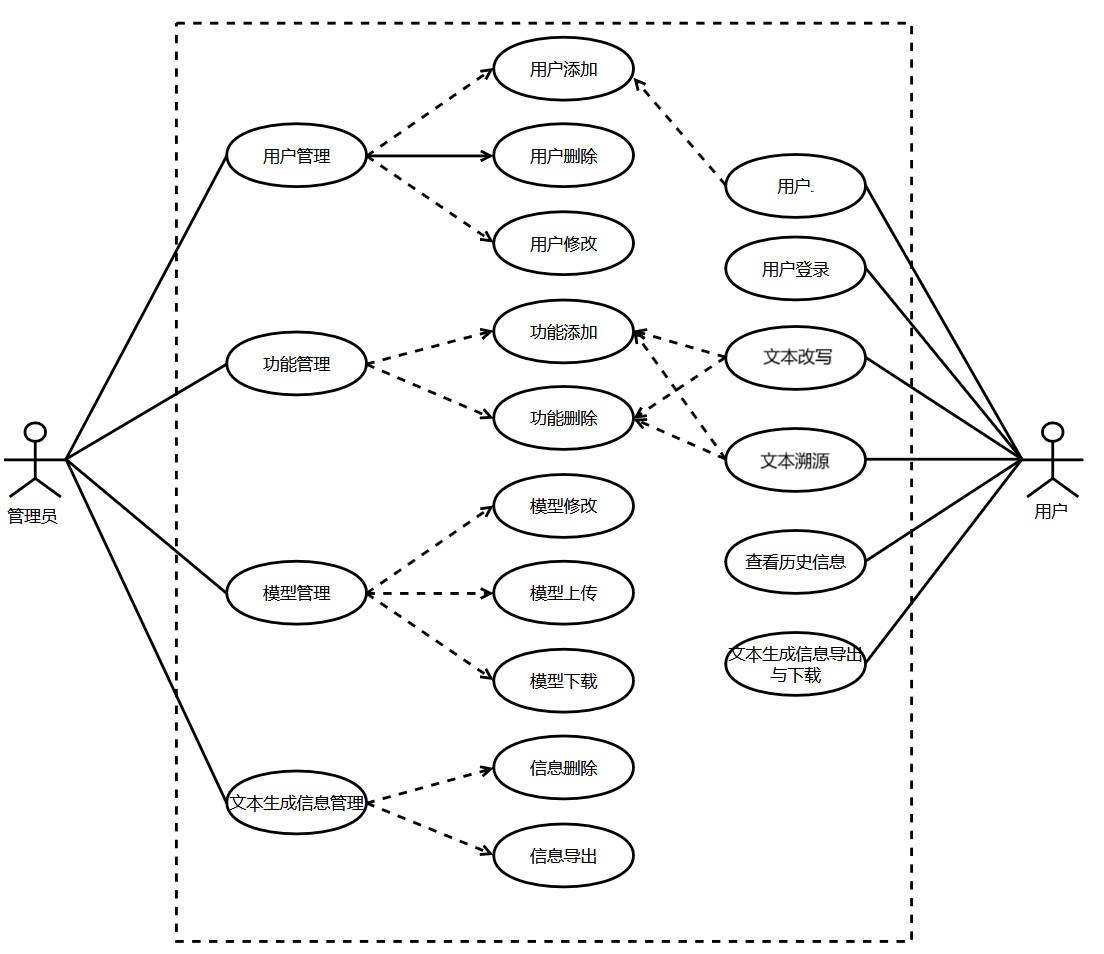
\includegraphics[width=\textwidth]{figures/sys-use-case.jpg}
    \caption{模型改写文本检测系统用例图}
    \label{fig:sys-use-case}
\end{figure*}

模型改写文本检测系统的总体用例图如图 \ref{fig:sys-use-case} 所示。

本系统用户功能需求分析如下:

\begin{enumerate}
\item \textbf{用户注册}:用户可以自行在系统上进行用户注册。
\item \textbf{用户登录}:用户可以使用已注册的账号密码登录系统。
\item \textbf{文本改写服务}:系统应当为用户提供文本改写服务,根据用户输入的文本,润色改写为流畅、通顺的文本。
\item \textbf{检测文本改写服务}:系统应当为用户提供检测某段文本是否被改写或由 AI 生成的服务,根据输入的源文本,得出检测结果。
\item \textbf{查看历史信息}:用户可以通过历史信息查询接口查看历史改写信息以及历史检测信息。
\item \textbf{文本生成信息导出与下载}:支持用户对文本信息进行导出并下载到本地。
\end{enumerate}

本系统管理员功能需求分析如下:

\begin{enumerate}
\item \textbf{用户管理}:管理员可以对用户进行添加、删除以及信息修改等操作。
\item \textbf{功能管理}:支持系统功能扩展,可以添加功能或者删除不需要的功能。
\item \textbf{模型管理}:管理员可以通过模型管理接口进行模型修改、上传和下载。
\item \textbf{文本生成信息管理}:对系统内冗余的文本信息进行删除或导出。
\end{enumerate}

\section{系统设计}
\label{sec:sys-design}

本章主要介绍模型改写文本检测系统的架构设计、模块和接口设计以及相关信息的数据库存储设计。

\subsection{系统架构设计}
\label{sec:sys-arch}

为了提高系统的灵活性、可扩展性和可维护性,本系统采用前后端分离的系统架构。前端只负责接收用户数据以及发送系统响应,后端提供具体的服务和处理逻辑,并将处理结果返回给前端。系统架构如图 \ref{fig:sys-arch} 所示,包括表现层、API 接口层、应用层、持久层以及基础层。

\begin{figure*}[htb]
    \centering
    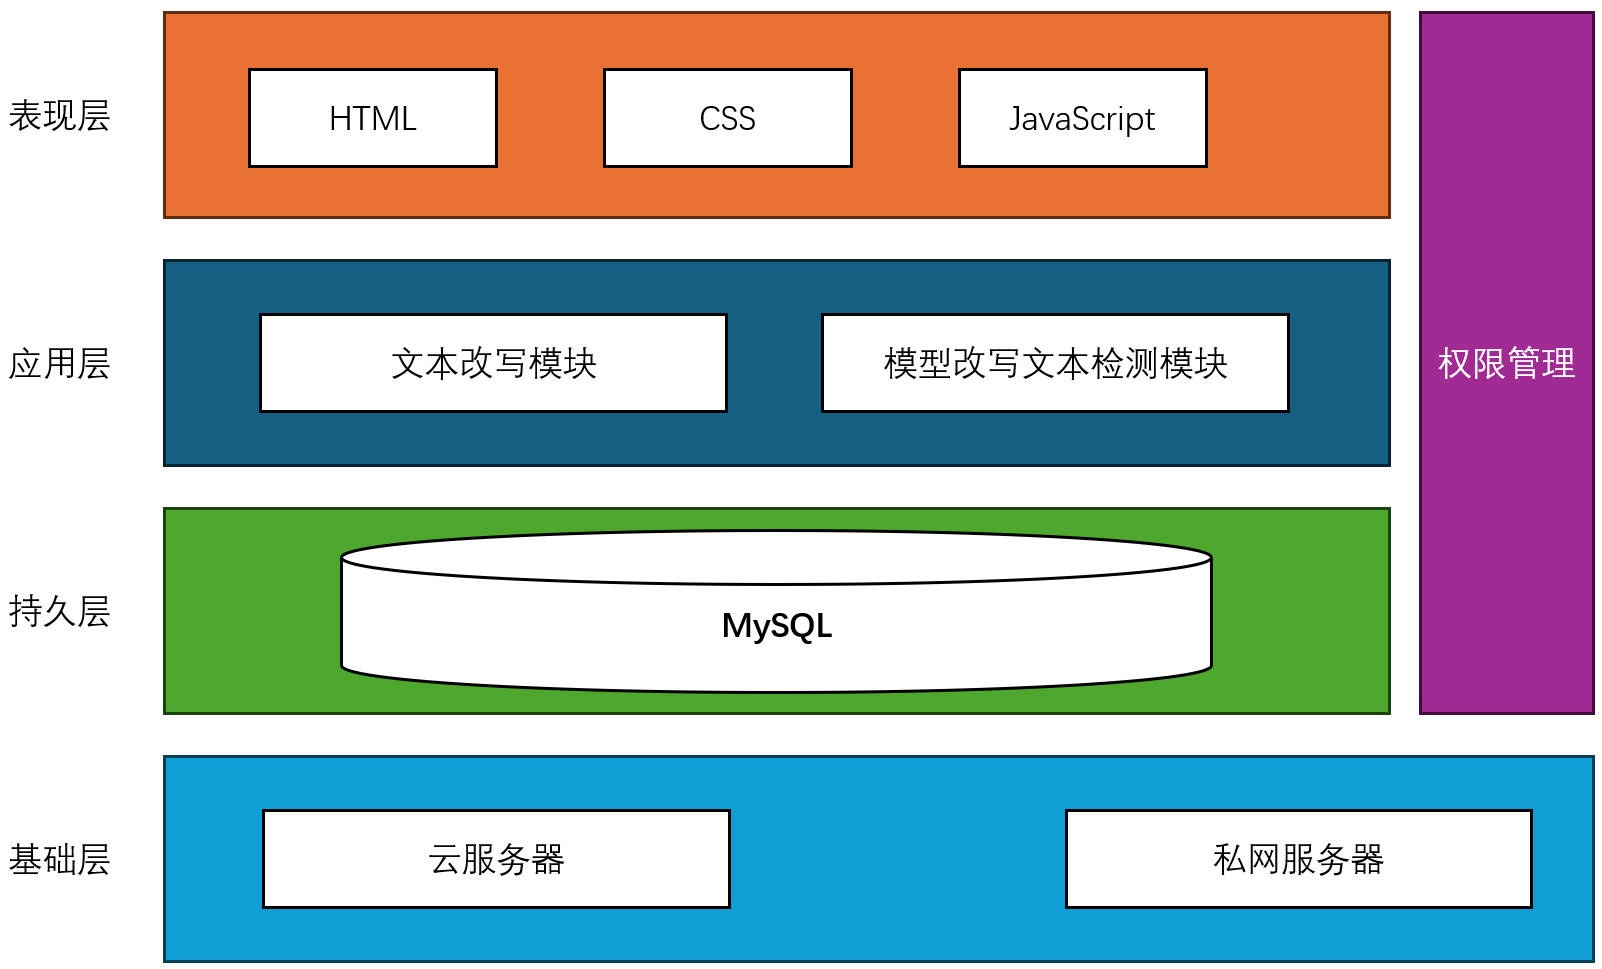
\includegraphics[width=\textwidth]{figures/sys-architecture.jpg}
    \caption{模型改写文本检测系统架构设计}
    \label{fig:sys-arch}
\end{figure*}

\begin{enumerate}
\item \textbf{表现层}:负责处理用户界面逻辑和交互控制,管理界面逻辑和权限控制,将系统数据以用户友好的方式展示,并实现用户交互。包括用户界面设计、页面布局和组件设计、样式设计和美化。使用 HTML 定义页面结构,CSS 美化页面样式,JavaScript处理页面交互和动态效果。

\item \textbf{API 接口层}:负责接收前端的请求并返回相应结果,使用 Nginx 进行反向代理,将外部请求转发给内部的服务器处理,并可以进行负载均衡,使系统能够处理大量请求并提供高性能的服务,Flask 应用程序接收到转发的请求后,执行相应的业务逻辑。通过独立的 API 接口层,前端和后端可以进行松耦合的交互,前端可以更灵活地调用后端的功能,而后端可以更容易地扩展和修改接口。

\item \textbf{应用层}:包含系统的核心业务逻辑,即对话生成模块以及机器翻译模块,另外提供用户管理服务、管理员管理服务等。将业务逻辑独立成应用层,可以使得不同功能模块的开发、测试和部署更加独立和灵活,同时也方便了后续的功能扩展和升级。

\item \textbf{数据层}:负责管理系统的数据存储和访问,使用 MySQL 存储用户账户信息、个人资料、权限和角色信息以及用户活动记录等结构化信息。使用 MongoDB 存储生成的文本内容等非结构化信息。通过独立的数据层,可以使得系统的数据访问更加统一和安全,同时也方便了数据的管理和维护。

\item \textbf{基础层}:使用云服务器和私网服务器部署系统,提供基础运行环境。

\end{enumerate}

通过采用前后端分离的系统架构,本系统能够实现前后端的松耦合、功能模块化
和独立部署,提高了系统的灵活性、可扩展性和可维护性,同时也提高了开发效率和
团队合作效率。

\subsection{模块和接口设计}
\label{sec:sys-module}

模型改写文本检测系统的模块和接口设计主要包括用户模块、管理员模块、文本改写模块和检测模型改写模块。每个模块都包含了相应的功能和接口设计,以满足系统的需求。

模型改写文本检测系统主要由用户模块、系统管理模块、和系统功能模块组成,模块间关系如图 \ref{fig:sys-module} 所示。用户模块主要负责用户的注册与登录,允许用户创建账户、密码管理并提供身份验证授权功能,保证用户能够正常访问和使用系统服务。系统管理模块主要负责功能管理、模型管理和数据管理,允许对系统功能进行灵活扩展,管理员可以添加新功能或者移除不再需要的功能,通过模型管理接口进行系统模型的修改、上传和下载,数据管理功能主要是对文本生成信息的管理,可以通过系统内的接口删除冗余的文本信息或将其导出下载到本地。系统功能模块是系统的核心,提供了各种具体的系统服务,用于处理前端接收的请求。系统功能包括对话生成和机器翻译,通该模块,用户可以与系统进行交互,请求特定或执行特定的任务,系统会根据接收到的请求,调用相应的功能模块来进行处理,并生成对应的响应。

\begin{figure*}[htb]
    \centering
    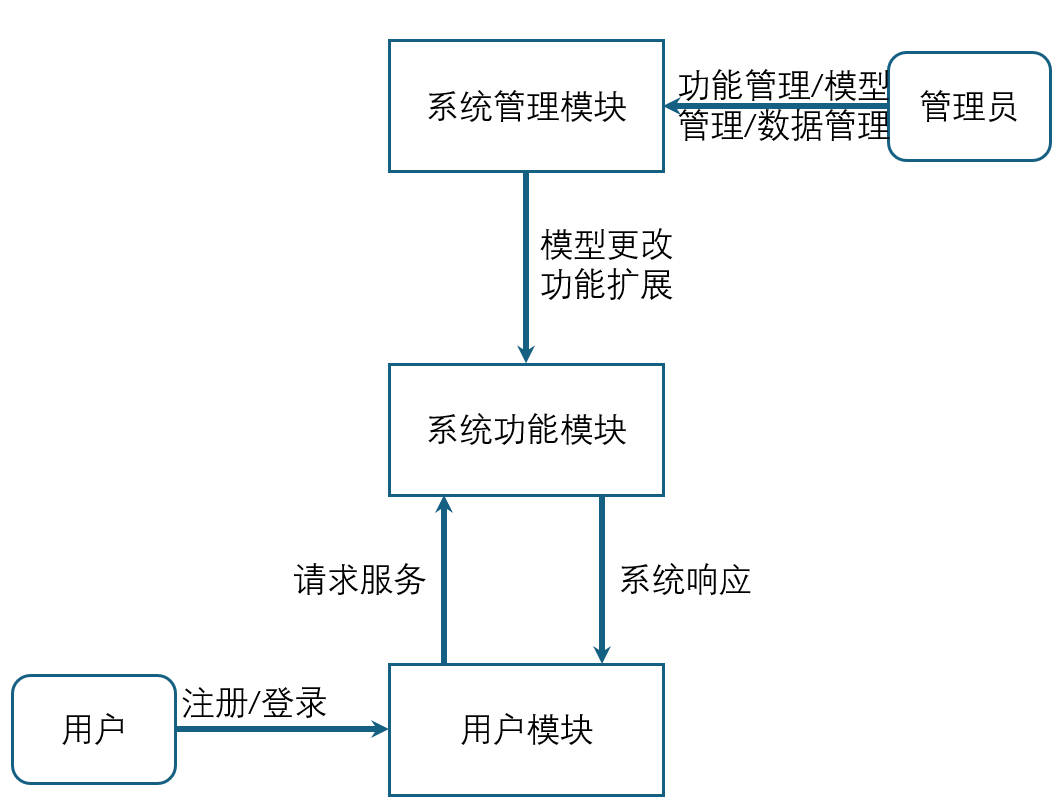
\includegraphics[width=0.8\textwidth]{figures/sys-module.jpg}
    \caption{模型改写文本检测系统模块设计}
    \label{fig:sys-module}
\end{figure*}

为了实现系统对用户的服务以及系统内不同模块之间数据传输,本章定义了系统核心接口,如表 \ref{tab:sys-interfaces} 所示。

\begin{table*}[htb]
    \centering
    \caption{模型改写文本检测系统核心接口说明}
    \label{tab:sys-interfaces}
    \begin{tabular}{cl}
        \toprule
        接口名 & 接口描述 \\
        \midrule
        userRegister & 接收用户提交注册信息,并进行用户注册。 \\
        userLogin & 接收用户提交登录信息,并进行身份验证和授权。 \\
        getModelInfo & 查询系统提供的模型,返回相关模型信息。 \\
        upLoadModel & 用于上传已训练好的模型到系统中,以供后续的服务需求。 \\
        downLoadModel & 用于从系统中导入已有模型。 \\
        funcDelete & 用于删除系统中不需要的功能。 \\
        funcCreate & 用于扩展系统功能,提供更好的服务。 \\
        dataManage & 用于管理系统中的文本生成信息,支持删除或下载文本数据。 \\
        dialogService & 接收用户输入,使用模型进行对话生成,并返回结果。 \\
        translationService & 接收用户输入,使用模型进行机器翻译,并返回结果。 \\
        \bottomrule
    \end{tabular}
\end{table*}

\subsection{数据库设计}
\label{sec:sys-db}

根据系统存储需求,本文采用 MySQL 数据库存储结构化数据,包括用户表、功能表、模型表、文本数据表等。

MySQL 数据库设计主要包括用户表、功能表、模型表和文本数据表。每个表都包含了相应的字段和数据类型,以满足系统的需求。

用户表:记录了用户 ID、用户名、密码、邮箱、权限、注册时间和最近登录时间信息,如表 \ref{tab:user-table} 所示。

\begin{table*}[htb]
    \centering
    \caption{用户表} \label{tab:user-table}
    \begin{tabular}{ccccc}
        \toprule
        \textbf{序号} & \textbf{字段} & \textbf{数据类型} & \textbf{说明} & \textbf{是否主键} \\
        \midrule
        1 & user\_id & int & 用户 ID & 是 \\
        2 & user\_name & varchar(30) & 用户名 & 否 \\
        3 & password & varchar(128) & 密码 & 否 \\
        4 & email & varchar(30) & 邮箱 & 否 \\
        5 & authority & enum & 权限 & 否 \\
        6 & register\_time & datetime & 注册时间 & 否 \\
        7 & lat\_login\_time & datetime & 最近登录时间 & 否 \\
        \bottomrule
    \end{tabular}
\end{table*}

功能表:记录了系统中相关功能的信息,包括功能 ID、功能名称以及功能接口,如表 \ref{tab:func-table} 所示。

\begin{table*}[htb]
    \centering
    \caption{功能表} \label{tab:func-table}
    \begin{tabular}{ccccc}
        \toprule
        \textbf{序号} & \textbf{字段} & \textbf{数据类型} & \textbf{说明} & \textbf{是否主键} \\
        \midrule
        1 & fuc\_id & int & 功能 ID & 是 \\
        2 & fuc\_name & varchar(30) & 功能名称 & 否 \\
        3 & fuc\_interface & varchar(30) & 功能接口 & 否 \\
        \bottomrule
    \end{tabular}
\end{table*}

模型表:记录系统中模型的相关信息,包括模型 ID、模型名称、模型类型以及模型上传时间,如表 \ref{tab:model-table} 所示。

\begin{table*}[htb]
    \centering
    \caption{模型表} \label{tab:model-table}
    \begin{tabular}{ccccc}
        \toprule
        \textbf{序号} & \textbf{字段} & \textbf{数据类型} & \textbf{说明} & \textbf{是否主键} \\
        \midrule
        1 & model\_id & int & 模型 ID & 是 \\
        2 & model\_name & varchar(20) & 模型名称 & 否 \\
        3 & model\_type & varchar(20) & 模型类型 & 否 \\
        4 & model\_size & varchar(20) & 模型大小 & 否 \\
        5 & upload\_time & datetime & 上传时间 & 否 \\
        \bottomrule
    \end{tabular}
\end{table*}

文本数据表:记录用户改写文本和模型改写文本信息,包括用户 ID、文本 ID、操作类型、操作时间、文本内容,如表 \ref{tab:text-table} 所示。

\begin{table*}[htbp]
    \centering
    \caption{文本数据表} \label{tab:text-table}
    \begin{tabular}{ccccc}
        \toprule
        \textbf{序号} & \textbf{字段} & \textbf{数据类型} & \textbf{说明} & \textbf{是否主键} \\
        \midrule
        1 & user\_id & int & 用户 ID & 是 \\
        2 & text\_id & int & 文本 ID & 是 \\
        3 & text\_type & varchar(20) & 操作类型 & 否 \\
        4 & generated\_time & datetime & 操作时间 & 否 \\
        5 & text\_content & text & 文本内容 & 否 \\
        \bottomrule
    \end{tabular}
\end{table*}

\section{系统实现}
\label{sec:sys-implement}

本节主要介绍模型改写文本检测系统的使用到的工具和系统服务,并分模块对系统功能进行讲解。

\subsection{开发环境与工具}
\label{sec:sys-env}

本文采用前后端分离架构进行开发,前端采用 Vue 来实现用户界面,提供良好的交互体验。后端开发采用 Pytorch、Transformers 等技术,用于构建文本生成服务。在编程语言方面,使用 HTML、CSS、JavaScript 和 Python,分别用于前端和后端的开发。为了提高开发效率,选择 Vscode 作为开发工具。在数据存储方面,系统使用了 MySQL 作为数据库,用于存储用户信息和生成的文本数据。为方便起见,使用 Flask 框架处理后端业务逻辑。为了保证系统安全, 采用 JWT 进行权限管理、验证用户身份。本文使用到的所有开发环境和工具如表 \ref{tab:sys-env} 所示。

\begin{table*}[htbp]
    \centering
    \caption{模型改写文本检测系统开发环境与工具}
    \label{tab:sys-env}
    \begin{tabular}{cc}
        \toprule
        \textbf{描述} & \textbf{配置} \\
        \midrule
        编程语言 & HTML、CSS、JavaScript、Python \\
        前端框架 & Vue \\
        服务端开发 & Pytorch1.8、Transformers \\
        开发工具 & Vscode \\
        数据库 & MySQL \\
        权限管理 & JWT \\
        服务器端 & Flask1.1.2、Docker \\
        \bottomrule
    \end{tabular}
\end{table*}

\section{系统展示}
\label{sec:sys-show}

由于管理员仅有在系统后台调用脚本进行管理操作,本文主要展示用户端的系统功能。用户端主要包括用户注册与登录、文本改写功能、检测模型改写功能和历史信息查询功能。用户注册与登录功能主要用于用户注册和登录系统,文本改写功能主要用于对输入的文本进行改写,检测模型改写功能主要用于检测输入的文本是否经过模型改写,历史信息查询功能主要用于查询用户的历史操作记录。

\subsection{用户注册与登录}

用户可以使用已注册的账号密码登录系统,如图 \ref{fig:sys-login} 所示。用户注册时需要填写用户名、密码和邮箱等信息,系统会对用户输入的信息进行验证,确保信息的合法性和完整性。如果未有注册账号,用户可以通过注册页面进行注册,如图 \ref{fig:sys-register} 所示。

\begin{figure*}[htb]
    \subfloat[listentry][用户登录]{
        \label{fig:sys-login}
        \centering
        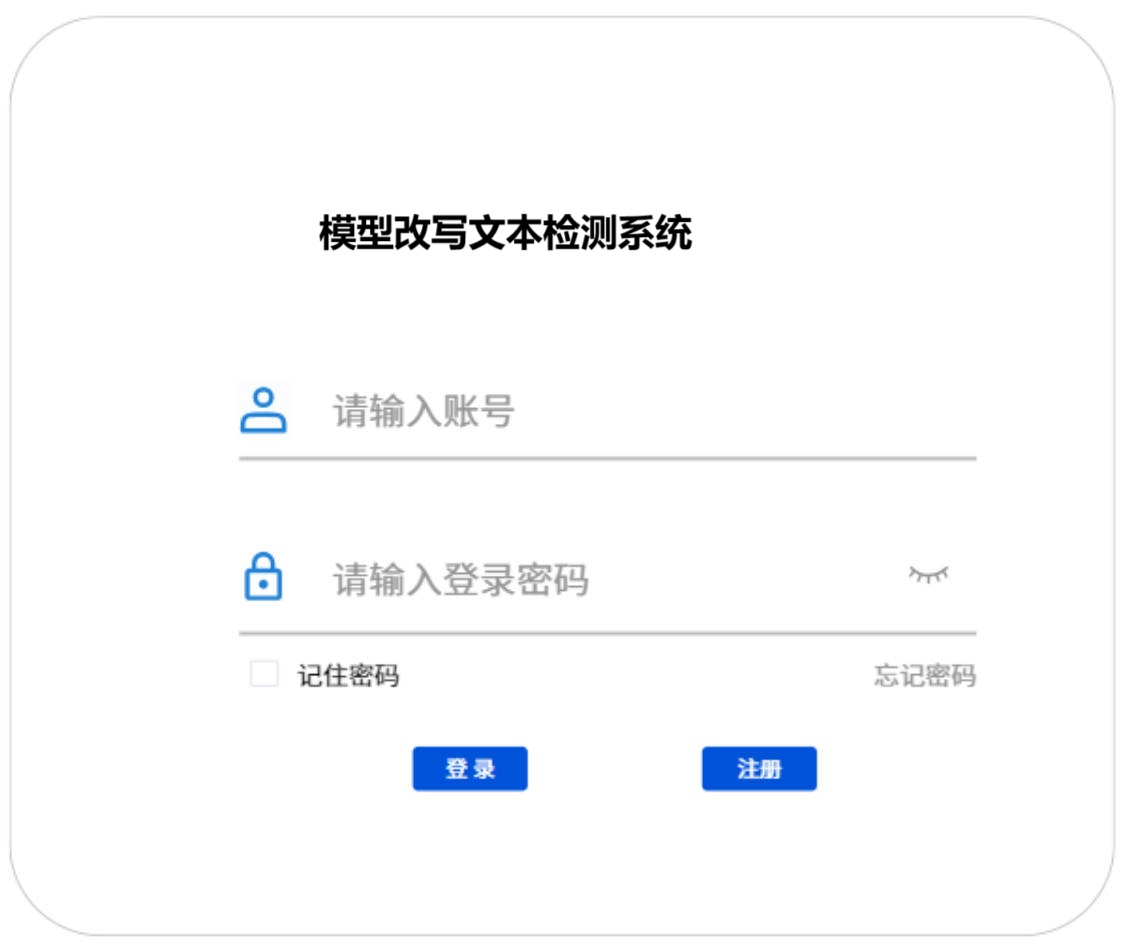
\includegraphics[width=0.45\textwidth]{figures/sys-login.jpg}
    }
    \hfill
    \subfloat[listentry][用户注册]{
        \label{fig:sys-register}
        \centering
        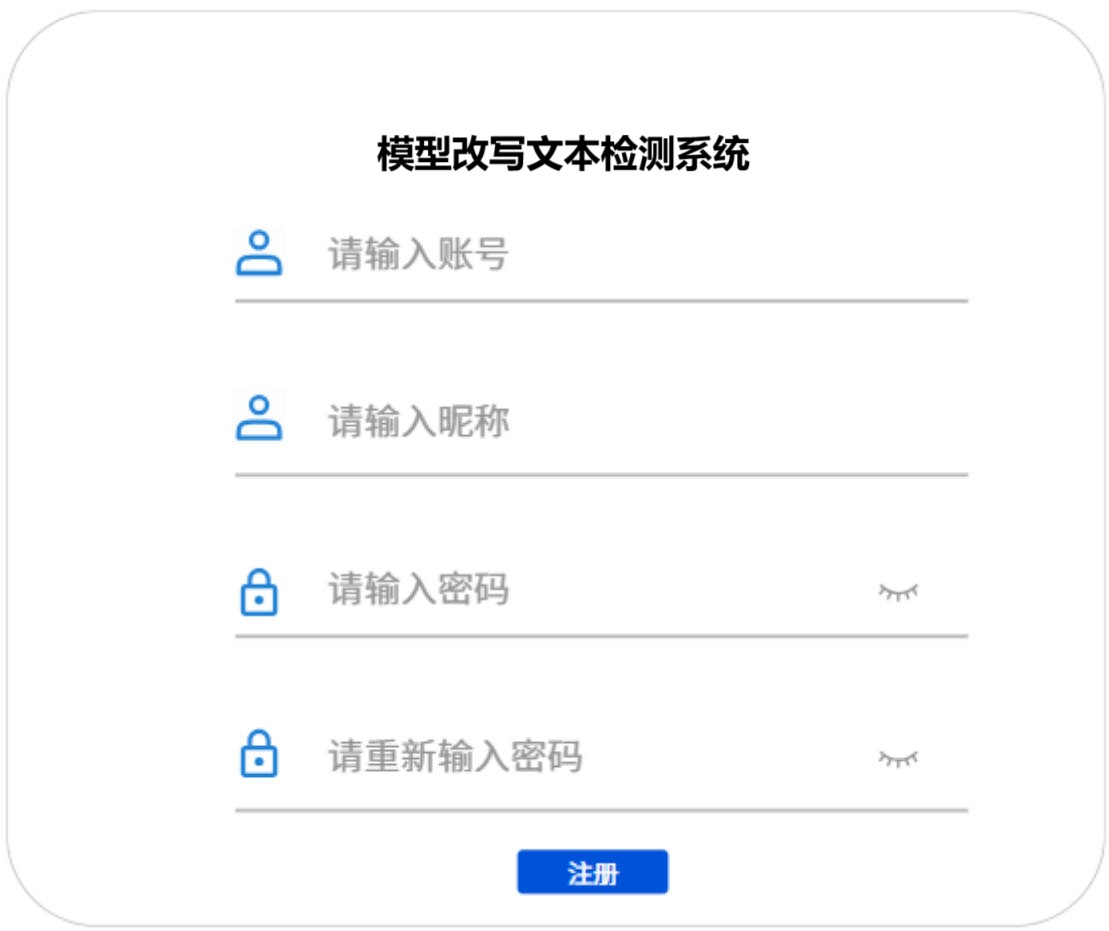
\includegraphics[width=0.45\textwidth]{figures/sys-register.jpg}
    }
    \caption{模型改写文本检测系统用户注册与登录}
    \label{fig:sys-login-register}
\end{figure*}

\subsection{文本改写功能}

用户登录后,可以在系统中进行文本改写操作,如图 \ref{fig:sys-polish} 所示。用户输入需要改写的文本,系统会使用模型进行改写,并返回改写后的文本。用户可以对改写后的文本进行查看和下载。用户可以选择不同的改写模型进行文本改写,系统会根据用户选择的模型进行相应的处理。用户还可以对改写后的文本进行编辑和修改,以满足自己的需求。

\begin{figure*}[htb]
    \centering
    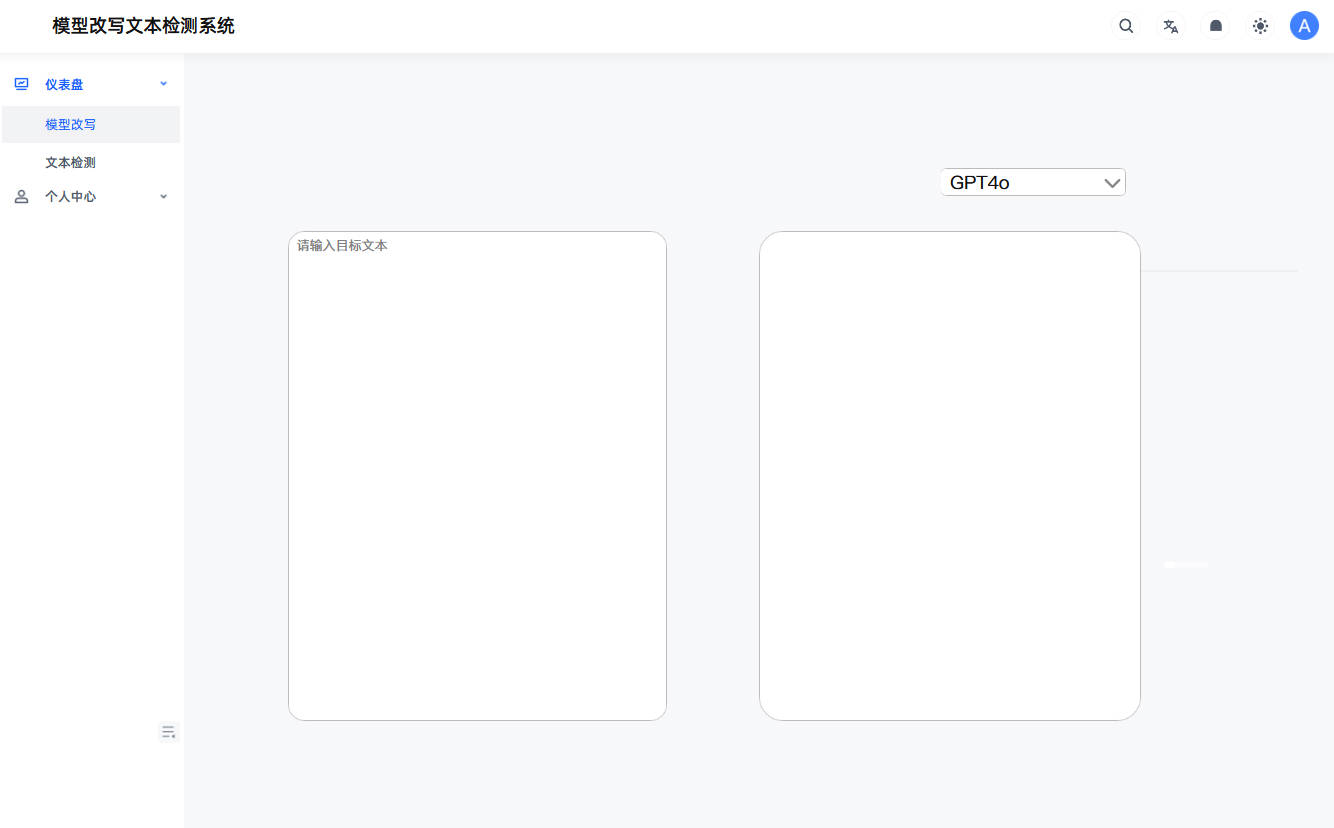
\includegraphics[width=\textwidth]{figures/sys-polish.jpg}
    \caption{模型改写文本检测系统——文本改写功能}
    \label{fig:sys-polish}
\end{figure*}

\subsection{模型改写文本检测功能}

用户登录后,可以在系统中进行模型改写文本检测操作,如图 \ref{fig:sys-detect} 所示。用户输入需要检测的文本,系统会使用模型进行检测,并返回检测结果。用户可以对检测结果进行查看和下载。用户还可以选择不同的检测模型进行文本检测,系统会根据用户选择的模型进行相应的处理。

\begin{figure*}[htb]
    \centering
    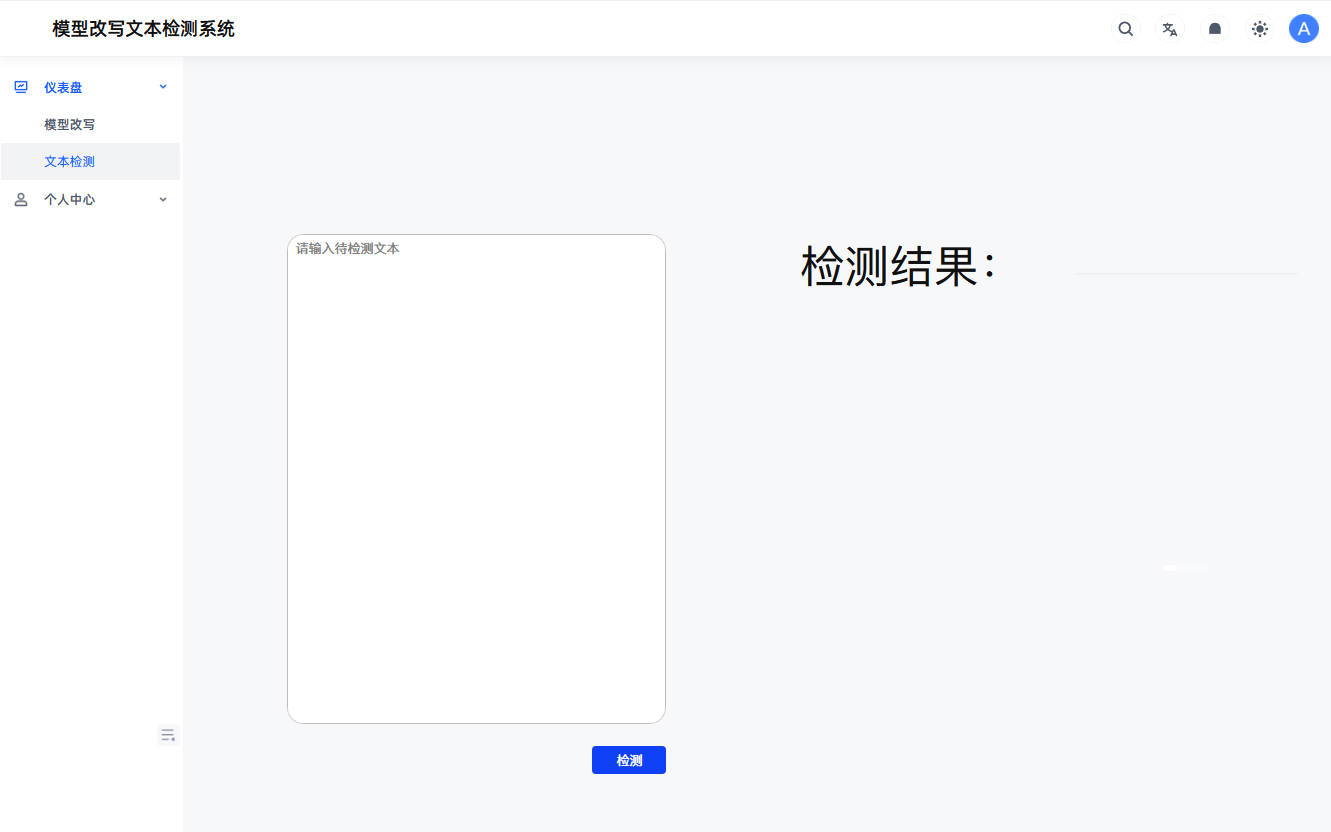
\includegraphics[width=\textwidth]{figures/sys-detect.jpg}
    \caption{模型改写文本检测系统——模型改写文本检测功能}
    \label{fig:sys-detect}
\end{figure*}

\section{本章小结}
\label{sec:sys-conclusion}

本章主要介绍了模型改写文本检测系统的设计与实现,包括需求分析、系统架构设计、模块和接口设计以及数据库设计。通过对系统的功能进行详细分析,明确了系统的业务需求和功能需求,为后续的系统实现提供了基础。系统采用前后端分离的架构设计,提高了系统的灵活性和可扩展性。通过模块和接口设计,明确了系统各个模块之间的关系和数据传输方式。数据库设计则为系统的数据存储提供了支持。最后,通过用户注册与登录、文本改写功能、模型改写文本检测功能等展示了系统的实际应用效果。

本章为模型改写文本检测系统的设计与实现奠定了基础,为后续的系统测试和优化提供了依据。通过对系统的设计与实现,可以看出模型改写文本检测系统在实际应用中的可行性和有效性,为后续的研究和应用提供了参考。